\documentclass[landscape]{article}
\usepackage[landscape,margin=0.7in]{geometry}
\usepackage{pgfplots}
\usepackage{tikz}
\pgfplotsset{compat=1.18}

\begin{document}
\pagestyle{empty}

\begin{figure}
    \centering
    \begin{tikzpicture}
        \begin{axis}[
            title={\Large Hybrid Strategy - Back Window Seats (t = 110)},
            xlabel={Seat Position},
            ylabel={Row Number},
            xtick={0,1,2,3,4,5},
            ytick={1,2,3,4,5,6,7},
            xtickmin=0,
            xtickmax=5,
            ytickmin=0.5,
            ytickmax=7.5,
            y dir=reverse,
            enlargelimits=false,
            axis on top,
            width=\textwidth,
            height=0.27\textheight,
            colorbar,
            colormap={boarding}{
                color(0)=(white);
                color(0.5)=(yellow);
                color(1)=(purple)
            },
            colorbar style={
                title={Status},
                ytick={0,0.5,1},
                yticklabels={Empty,Boarding,Seated},
            },
            point meta min=0,
            point meta max=1
        ]
            
        % Back window seats boarding pattern
        \addplot[matrix plot, mesh/cols=6, point meta=explicit] table [meta=C] {
            x y C
            0 1 0
            1 1 0
            2 1 0
            3 1 0
            4 1 0
            5 1 0
            0 2 0
            1 2 0
            2 2 0
            3 2 0
            4 2 0
            5 2 0
            0 3 0
            1 3 0
            2 3 0
            3 3 0
            4 3 0
            5 3 0
            0 4 0
            1 4 0
            2 4 0
            3 4 0
            4 4 0
            5 4 0
            0 5 1
            1 5 0
            2 5 0
            3 5 0
            4 5 0
            5 5 1
            0 6 1
            1 6 0
            2 6 0
            3 6 0
            4 6 0
            5 6 1
            0 7 0.5
            1 7 0
            2 7 0
            3 7 0
            4 7 0
            5 7 0.5
        };
        
        % Draw aisle line
        \draw[black, thick, dashed] (axis cs:2.5,0.5) -- (axis cs:2.5,7.5);
        
        % Draw zone boundaries
        \fill[blue!20, opacity=0.3] (axis cs:-0.5,4.5) rectangle (axis cs:5.5,7.5);
        
        % Seat type markers at the bottom
        \node[font=\small] at (axis cs:0,-1) {Window};
        \node[font=\small] at (axis cs:1,-1) {Middle};
        \node[font=\small] at (axis cs:2,-1) {Aisle};
        \node[font=\small] at (axis cs:3,-1) {Aisle};
        \node[font=\small] at (axis cs:4,-1) {Middle};
        \node[font=\small] at (axis cs:5,-1) {Window};
        
        % Colored bars under seat types
        \fill[green!70!black] (axis cs:-0.5,-1.3) rectangle (axis cs:0.5,-0.7);
        \fill[green!70!black] (axis cs:4.5,-1.3) rectangle (axis cs:5.5,-0.7);
        
        % Zone labels
        \node[right] at (axis cs:5.5,6) {Back (Current)};
        \node[right] at (axis cs:5.5,3) {Middle};
        \node[right] at (axis cs:5.5,1.5) {Front};
        
        % Time indicator
        \node[font=\Large] at (axis cs:2.5,-2) {t = 110 seconds};
        
        % Description
        \node[draw, align=left, anchor=south west] at (axis cs:-0.5,8.5) {
            \textbf{Hybrid Boarding Strategy:}\\
            • Combines elements of both back-to-front and outside-in strategies\\
            • Aircraft divided into three zones: Back, Middle, Front\\
            • Boarding sequence: Back window → Middle window → Front window → Back middle → etc.\\
            • Currently boarding: Back window seats\\
            • Current status: Initial phase
        };
        \end{axis}
    \end{tikzpicture}
\end{figure}

\begin{figure}
    \centering
    \begin{tikzpicture}
        \begin{axis}[
            title={\Large Hybrid Strategy - Middle Seats Phase (t = 220)},
            xlabel={Seat Position},
            ylabel={Row Number},
            xtick={0,1,2,3,4,5},
            ytick={1,2,3,4,5,6,7},
            xtickmin=0,
            xtickmax=5,
            ytickmin=0.5,
            ytickmax=7.5,
            y dir=reverse,
            enlargelimits=false,
            axis on top,
            width=\textwidth,
            height=0.27\textheight,
            colorbar,
            colormap={boarding}{
                color(0)=(white);
                color(0.5)=(yellow);
                color(1)=(purple)
            },
            colorbar style={
                title={Status},
                ytick={0,0.5,1},
                yticklabels={Empty,Boarding,Seated},
            },
            point meta min=0,
            point meta max=1
        ]
            
        % Middle seats phase boarding pattern
        \addplot[matrix plot, mesh/cols=6, point meta=explicit] table [meta=C] {
            x y C
            0 1 1
            1 1 0
            2 1 0
            3 1 0
            4 1 0
            5 1 1
            0 2 1
            1 2 0
            2 2 0
            3 2 0
            4 2 0
            5 2 1
            0 3 1
            1 3 0.5
            2 3 0
            3 3 0
            4 3 0.5
            5 3 1
            0 4 1
            1 4 0
            2 4 0
            3 4 0
            4 4 0
            5 4 1
            0 5 1
            1 5 1
            2 5 0
            3 5 0
            4 5 1
            5 5 1
            0 6 1
            1 6 0.5
            2 6 0
            3 6 0
            4 6 0.5
            5 6 1
            0 7 1
            1 7 0
            2 7 0
            3 7 0
            4 7 0
            5 7 1
        };
        
        % Draw aisle line
        \draw[black, thick, dashed] (axis cs:2.5,0.5) -- (axis cs:2.5,7.5);
        
        % Draw zone boundaries
        \fill[blue!20, opacity=0.3] (axis cs:-0.5,2.5) rectangle (axis cs:5.5,4.5);
        
        % Seat type markers at the bottom
        \node[font=\small] at (axis cs:0,-1) {Window};
        \node[font=\small] at (axis cs:1,-1) {Middle};
        \node[font=\small] at (axis cs:2,-1) {Aisle};
        \node[font=\small] at (axis cs:3,-1) {Aisle};
        \node[font=\small] at (axis cs:4,-1) {Middle};
        \node[font=\small] at (axis cs:5,-1) {Window};
        
        % Colored bars under seat types
        \fill[green!70!black] (axis cs:-0.5,-1.3) rectangle (axis cs:0.5,-0.7);
        \fill[green!70!black] (axis cs:4.5,-1.3) rectangle (axis cs:5.5,-0.7);
        
        \fill[orange!70!black] (axis cs:0.5,-1.3) rectangle (axis cs:1.5,-0.7);
        \fill[orange!70!black] (axis cs:3.5,-1.3) rectangle (axis cs:4.5,-0.7);
        
        % Zone labels
        \node[right] at (axis cs:5.5,6) {Back (Complete)};
        \node[right] at (axis cs:5.5,3.5) {Middle (Current)};
        \node[right] at (axis cs:5.5,1.5) {Front};
        
        % Time indicator
        \node[font=\Large] at (axis cs:2.5,-2) {t = 220 seconds};
        
        % Description
        \node[draw, align=left, anchor=south west] at (axis cs:-0.5,8.5) {
            \textbf{Hybrid Boarding Strategy:}\\
            • All window seats in back zone completed\\
            • All window seats in middle and front zones completed\\
            • Currently boarding: Middle seats in middle zone\\
            • Systematic approach with minimal passenger interference\\
            • Current status: Middle phase
        };
        \end{axis}
    \end{tikzpicture}
\end{figure}

\begin{figure}
    \centering
    \begin{tikzpicture}
        \begin{axis}[
            title={\Large Hybrid Strategy - Final Phase (t = 330)},
            xlabel={Seat Position},
            ylabel={Row Number},
            xtick={0,1,2,3,4,5},
            ytick={1,2,3,4,5,6,7},
            xtickmin=0,
            xtickmax=5,
            ytickmin=0.5,
            ytickmax=7.5,
            y dir=reverse,
            enlargelimits=false,
            axis on top,
            width=\textwidth,
            height=0.27\textheight,
            colorbar,
            colormap={boarding}{
                color(0)=(white);
                color(0.5)=(yellow);
                color(1)=(purple)
            },
            colorbar style={
                title={Status},
                ytick={0,0.5,1},
                yticklabels={Empty,Boarding,Seated},
            },
            point meta min=0,
            point meta max=1
        ]
            
        % Final phase boarding pattern
        \addplot[matrix plot, mesh/cols=6, point meta=explicit] table [meta=C] {
            x y C
            0 1 1
            1 1 1
            2 1 0.5
            3 1 0.5
            4 1 1
            5 1 1
            0 2 1
            1 2 1
            2 2 1
            3 2 1
            4 2 1
            5 2 1
            0 3 1
            1 3 1
            2 3 1
            3 3 1
            4 3 1
            5 3 1
            0 4 1
            1 4 1
            2 4 0.5
            3 4 0.5
            4 4 1
            5 4 1
            0 5 1
            1 5 1
            2 5 1
            3 5 1
            4 5 1
            5 5 1
            0 6 1
            1 6 1
            2 6 1
            3 6 1
            4 6 1
            5 6 1
            0 7 1
            1 7 1
            2 7 0.5
            3 7 0.5
            4 7 1
            5 7 1
        };
        
        % Draw aisle line
        \draw[black, thick, dashed] (axis cs:2.5,0.5) -- (axis cs:2.5,7.5);
        
        % Draw zone boundaries
        \fill[blue!20, opacity=0.3] (axis cs:-0.5,0.5) rectangle (axis cs:5.5,2.5);
        
        % Seat type markers at the bottom
        \node[font=\small] at (axis cs:0,-1) {Window};
        \node[font=\small] at (axis cs:1,-1) {Middle};
        \node[font=\small] at (axis cs:2,-1) {Aisle};
        \node[font=\small] at (axis cs:3,-1) {Aisle};
        \node[font=\small] at (axis cs:4,-1) {Middle};
        \node[font=\small] at (axis cs:5,-1) {Window};
        
        % Colored bars under seat types
        \fill[green!70!black] (axis cs:-0.5,-1.3) rectangle (axis cs:0.5,-0.7);
        \fill[green!70!black] (axis cs:4.5,-1.3) rectangle (axis cs:5.5,-0.7);
        
        \fill[orange!70!black] (axis cs:0.5,-1.3) rectangle (axis cs:1.5,-0.7);
        \fill[orange!70!black] (axis cs:3.5,-1.3) rectangle (axis cs:4.5,-0.7);
        
        \fill[red!70!black] (axis cs:1.5,-1.3) rectangle (axis cs:2.5,-0.7);
        \fill[red!70!black] (axis cs:2.5,-1.3) rectangle (axis cs:3.5,-0.7);
        
        % Zone labels
        \node[right] at (axis cs:5.5,6) {Back (Complete)};
        \node[right] at (axis cs:5.5,3.5) {Middle (Complete)};
        \node[right] at (axis cs:5.5,1.5) {Front (Current)};
        
        % Time indicator
        \node[font=\Large] at (axis cs:2.5,-2) {t = 330 seconds};
        
        % Description
        \node[draw, align=left, anchor=south west] at (axis cs:-0.5,8.5) {
            \textbf{Hybrid Boarding Strategy:}\\
            • All window and middle seats completed in all zones\\
            • All aisle seats in back and middle zones completed\\
            • Currently boarding: Final aisle seats in front zone\\
            • Combines efficiency of both strategies\\
            • Estimated total boarding time: 10.0 minutes
        };
        \end{axis}
    \end{tikzpicture}
\end{figure}

\end{document}